\begin{bibunit}[IEEEtran.bst]

\clearemptydoublepage
\chapter{Titre du premier chapitre}
\label{chap:1}

Lorem ipsum dolor sit amet, consectetuer adipiscing elit. Maecenas fermentum, elit non lobortis cursus, orci velit suscipit est, id mollis turpis mi eget orci.

\section{Première section du chapitre}

Lorem ipsum dolor sit amet, consectetuer adipiscing elit. Maecenas fermentum, elit non lobortis cursus, orci velit suscipit est, id mollis turpis mi eget orci.

\subsection{Première sous-section}

Lorem ipsum dolor sit amet, consectetuer adipiscing elit. Maecenas fermentum, elit non lobortis cursus, orci velit suscipit est, id mollis turpis mi eget orci.

Voir figure \ref{fig:mafigure2}.


\begin{figure}[htbp]
   \begin{center}
      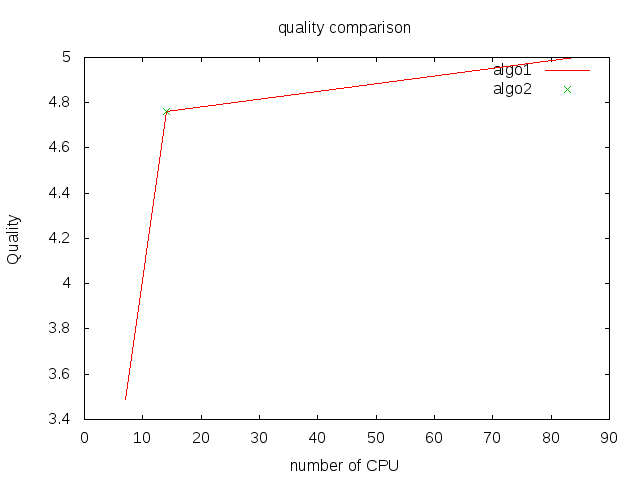
\includegraphics[width=0.8\linewidth]{Chapitre1/Ch1-Figures/comparison.png}
   \end{center}
   \caption[titre court pour la liste des figures]
   {\footnotesize Titre plus long avec des explications.}
   \label{fig:mafigure2}
\end{figure}

\subsection{Deuxième sous-section}

Lorem ipsum dolor sit amet, consectetuer adipiscing elit. Maecenas fermentum, elit non lobortis cursus, orci velit suscipit est, id mollis turpis mi eget orci.

\section{Conclusion du premier chapitre}

Lorem ipsum dolor sit amet, consectetuer adipiscing elit. Maecenas fermentum, elit non lobortis cursus, orci velit suscipit est, id mollis turpis mi eget orci.

In this manuscript I'd like to cite \cite{remo3,remo4}.

\addcontentsline{toc}{section}{Bibliography}
\putbib[./Chapitre1/Ch1-Biblio.bib]
\end{bibunit}
